\documentclass[lettersize,journal,english]{IEEEtran}
\usepackage[T1]{fontenc}
\usepackage[utf8]{inputenc}
\usepackage{amsmath,amsfonts,amssymb}
\usepackage{algorithmic}
\usepackage{algorithm}
\usepackage{array}
\usepackage[caption=false,font=normalsize,labelfont=sf,textfont=sf]{subfig}
\usepackage{textcomp}
\usepackage{stfloats}
\usepackage{url}
\usepackage{verbatim}
\usepackage{graphicx}
\usepackage{cite}
\usepackage{booktabs}
\usepackage{units}
\usepackage[unicode=true,pdfusetitle,
 bookmarks=true,bookmarksnumbered=false,bookmarksopen=false,
 breaklinks=false,pdfborder={0 0 0},pdfborderstyle={},backref=false,colorlinks=true]{hyperref}
\hypersetup{
 urlcolor=blue, linkcolor=black}
\usepackage[acronym]{glossaries}
\hyphenation{op-tical net-works semi-conduc-tor IEEE-Xplore}

\global\long\def\BDsites{\textsf{BD\_sites}}

\title{Adaptative neigbouring methods applied to telephonic base stations}
\author{\IEEEauthorblockN{Paul MÉHAUD}\\
\IEEEauthorblockA{\textit{Intern at CTU in Prague} \\
\textit{INSA Rouen Normandie}\\
paul.mehaud@insa-rouen.fr}\\
\and
\IEEEauthorblockN{Brendan SÉVELLEC}\\
\IEEEauthorblockA{\textit{Intern at CTU in Prague} \\
\textit{INSA Rouen Normandie}\\
brendan.sevellec@insa-rouen.fr}}

\makeglossaries

\setglossarypreamble{All definitions are from \href{https://www.dictionary.com/}{Dictionnary.com}}

\newglossaryentry{base station}
{
    name=base station,
    description={A fixed transmitter that forms part of an otherwise mobile radio network}
}

\newglossaryentry{convHull}
{
    name=convex hull,
    description={The smallest convex set containing a given set}
}



\newacronym{arcep}{ARCEP}{French Regulatory Authority for Electronic Communications and Posts}
\newacronym{anfr}{ANFR}{French National Frequency Agency}
\newacronym{bs}{BS}{\Gls{base station}}
\newacronym{dbscan}{DBScan}{Density-Based Spatial Clustering of Applications with Noise}
\newacronym{hdbscan}{HDBScan}{Hierarchical Density-Based Spatial Clustering of Applications with Noise}

\usepackage[english,french]{babel}

\begin{document}
\selectlanguage{english}
\maketitle

\begin{abstract}
    The field of telecommunication represents a gigantic mine of information, the smartphone penetration rate being 69\%
    in 2023 in the world, and 97\% in France. Therefore, the collected datas represent a big opportunity for telecommunication
    companies to predict their customers behaviour for internal or marketing purposes. Thus, it is primordial for these companies
    to be able to determine if a user is moving. For that, it is necessary to understand the neighbouring relationships between the 
    telephonic base stations. This article aims at proposing and comparing different method, that aim at adaptively detect these
    relationship between telephonic base stations. Therefore, it proposes a new method to create a neighbouring graph of base
    stations via their geographical positions.
\end{abstract}

\section{Introduction}
    \IEEEPARstart{T}{his} article articulates around the themes of mobile networks and neighbouring problems. 

    A cellular network, also know as a mobile network, is a type of telecommunications network that is dispersed over geographical areas known 
    as cells, each of which is supplied by at least one fixed-location transceiver called base station. These base stations give the cell network
    coverage so that voice, data, and other kinds of content may be transmitted.
    
    Given a list of points and their coordinates, a neighbouring problem consists in finding, for each point, a list of other points that are 
    considered as its neighbours.

    
\section{Related works}

\section{Databases}
\noindent Several databases have been used in order to test the different aspects of the methods. However, one of
them is directly necessary to the method itself.

\subsection{Main database}
This database \cite{main_database} contains all the information needed for the application of the method. It is from
\acrfull{arcep}, which is an independent French administrative authority responsible for regulating electronic and postal 
communications and press distribution.

This database was first published for the third quarter of 2017 and the version we are using was published on 28\textsuperscript{th} March 2024 \cite{main_database_hist}.
It's updated for every quarter. For instance, the data we used refers to the fourth quarter of 2023.

It consists of a substantial collection of $108\,838$ entries, encompassing $29$ distinct features of a size of $\unit[16.7]{Mo}$.
Each row of the database corresponds to detailed information regarding a specific BS. For the scope of this study,
our analysis will focus on the fields outlined in Table~\ref{table:data_columns}.
\begin{table}
    \centering
    \caption{Description of the main database columns used in the experiments}
    \label{table:data_columns}
    \begin{tabular}{ll}
        \toprule
        \textbf{Column} & \textbf{Description} \\
        \cmidrule(lr){1-2}
        \textsl{id\_station\_anfr} & \acrshort{anfr} \acrshort{bs} ID \\ 
        \textsl{nom\_op} & Name of the provider \\
        \textsl{$x$, $y$, latitude, longitude} & Base station coordinates \\ 
        \textsl{nom\_reg, nom\_dep, nom\_com} & Additional location information \\  
        \textsl{site\_2g, 3g, 4g, 5g} & Technology used by the \acrshort{bs} \\ 
        \bottomrule
    \end{tabular}
\end{table}

For station coordinates, we will use two different reference points: $x$ and $y$ coordinates, which are Lambert-93 projections of latitude and longitude.
This dual system has two advantages: the $x$, $y$ coordinates allow us to calculate distances in meters using the Euclidean norm,
which is more efficient in terms of calculation, and the GPS coordinates make it easier to display the points on a map.

In addition, we can find in the columns the name of the provider (\textsl{nom\_op}). In this database, only the four main french providers are represented:
\emph{Bouygues Telecom}, \emph{Free Mobile}, \emph{Orange} and \emph{SFR}.

Finally, we have informations about the technologies used in every site. Indeed, a site can use multiple technologies.
In Figure~\ref{fig:data_evolution} you will find the evolution of each technology from the first updates of the data.
\begin{figure}
    \centering
    \boxed{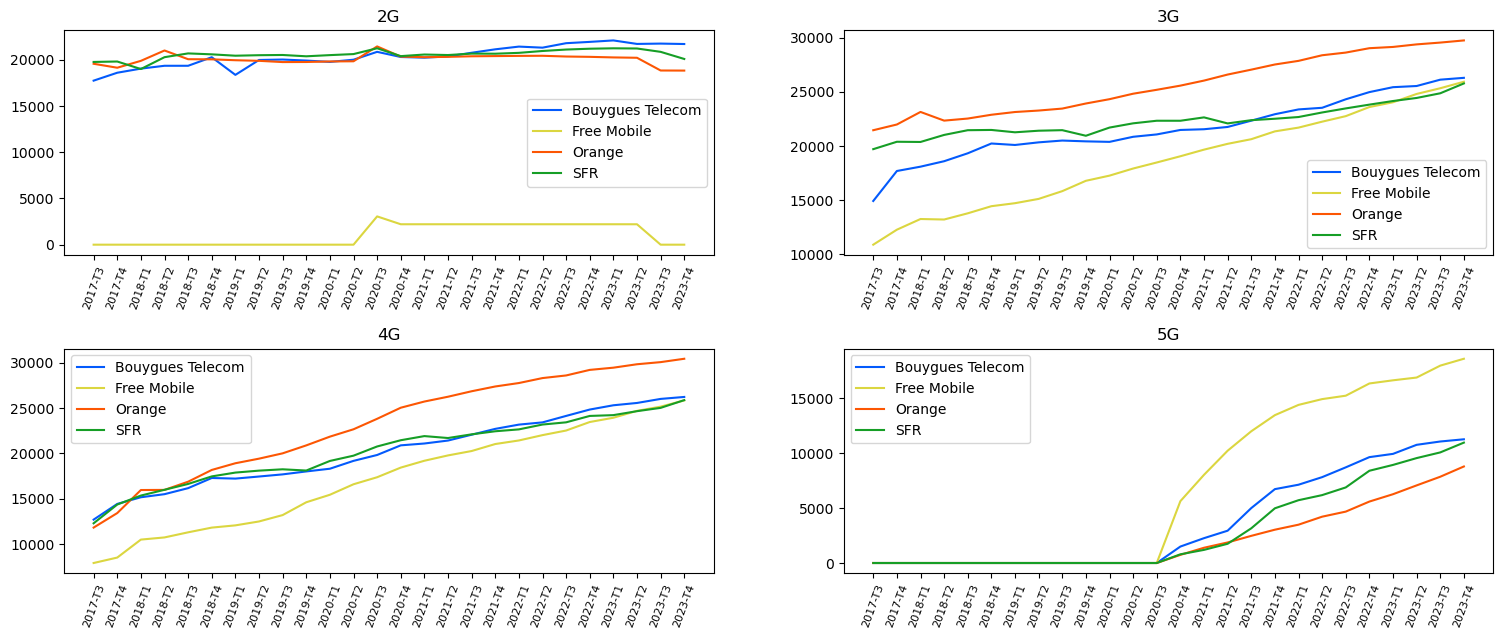
\includegraphics[width=2.5in]{images/data_analysis/technos-evolution.png}}
    \caption{Evolution by quarter year and by technology of the number of \acrshort{bs}}
    \label{fig:data_evolution}
\end{figure}
Then, in Figure~\ref{fig:data_technos} you will find a chart showing the number of times each technology is present for each provider.
\begin{figure}
    \centering
    \boxed{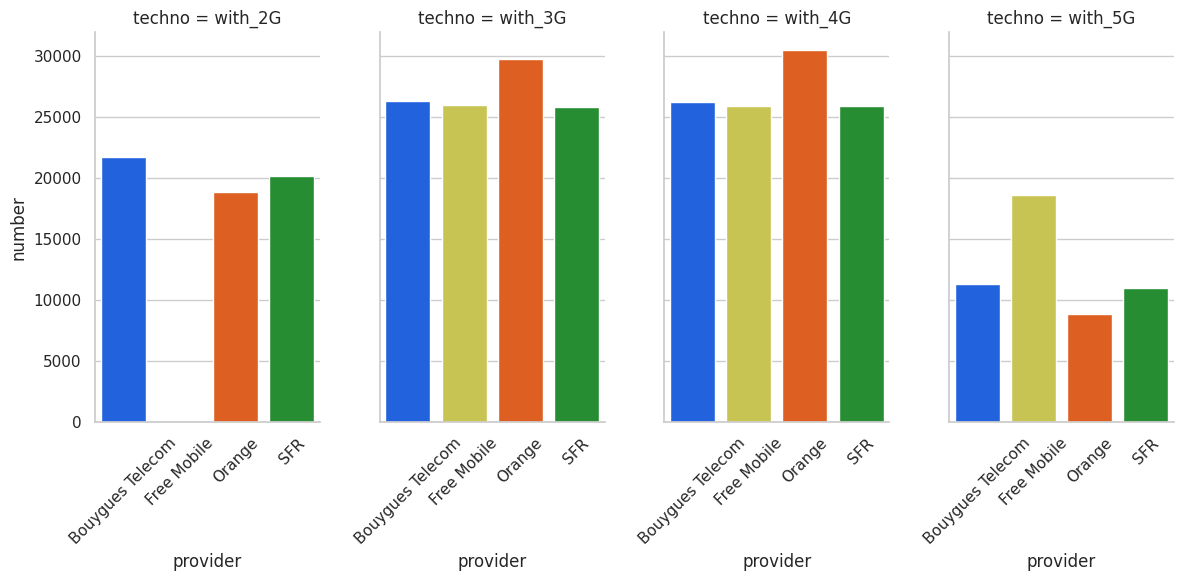
\includegraphics[width=2.5in]{images/data_analysis/with_techno.png}}
    \caption{Breakdown, by operator, of the number of sites containing a given technology}
    \label{fig:data_technos}
\end{figure}
We can see, for example, that \emph{Free Mobile} doesn't have any base station with $2$G technology. Additionally, you can als find these values in Table~\ref{table:techno_numbers}.
\begin{table}
    \centering
    \caption{Number of \acrfull{bs} equipped, at least, with $x$G, by provider}
    \label{table:techno_numbers}
    \begin{tabular}{cccccc}
        \toprule
        \textbf{Technology} & \textbf{Bouygues} & \textbf{Free} & \textbf{Orange} & \textbf{SFR} & \textbf{Total} \\
        \cmidrule(lr){1-6}
        \textbf{2G} & 21710 & 0 & 18835 & 20093 & 60638 \\
        \textbf{3G} & 26294 & 25934 & 29748 & 25777 & 107753 \\
        \textbf{4G} & 26231 & 25847 & 30440 & 25881 & 108399 \\
        \textbf{5G} & 11271 & 18607 & 8794 & 10968 & 49640 \\
        \textbf{Total} & 26331 & 25949 & 30540 & 26018 & 108838 \\
        \bottomrule
    \end{tabular}
\end{table}

\subsection{Filtering the main database}
As seen before this database is really huge, as a matter of fact we will only work on a portion of it.

Firstly, only one provider will be kept because a \acrshort{bs} from provider $x$ can't be considered as a neighbour of \acrshort{bs} from provider $y$.
Consequently, we have chosen \emph{Orange} because it is the one that has the largest number of \acrshort{bs}.

Secondly, for the same reasons as before, only one technology is kept. Thus, we kept all \acrshort{bs} using, at least, 4G.

In order to simplify the calculation times, the vision and the assessment of the quality of the results, we will only work on sites located in the Normandy region.
This is because Normandy is where our school is based, giving us a better view of its geography.

\subsection{Additional database}
In order to compare the results of city detection, we needed a reference database. We therefore used the population data provided by INSEE.
[Pas sur de l'utilité de présenter cette base en fait, ptet juste la principale suffit]

\section{Reminder on existing methods\label{sec:reminder}}
\subsection{Finding potential neighbours}
When we are looking for neighbours, we need, at first, a list of potential neighbours for each point.
For that, we will construct a neigbouring graph $G = (P, U)$ where $P$ is the set of all points and each edge in $U$ represents a neighbouring relation.

\subsubsection{$k$-NN graph}
The most intuitive method is to connect each point to its $k$ nearest neighbours, where $k \in \mathbb{N}^*$ is a parameter to be fixed. 

However, this method can be criticised, because it always finds $k$ neighbours for each point, no matter the reality of the 
data.

\subsubsection{Delaunay triangulation}
A Delaunay triangulation \cite{art_delaunay} of a set of points in the plane subdivides their \gls{convHull} into triangles whose circumcircles 
do not contain any of the points.

A Voronoi diagram is a tessellation pattern in which $n$ points scattered on a plane subdivides in 
exactly $n$ cells enclosing a portion of the plane that is closest to each point. 

It is a well-known method when trying to find neighbours \cite{delaunay_neighbor}
since a Delaunay triangulation is the pendant of a Voronoi diagram, cf. Figure~\ref{fig:del_tri}, i.e. two points are connected in the
Delaunay triangulation if their associated cells are touching each other in the Voronoi diagram.

\begin{figure}
    \centering
    \boxed{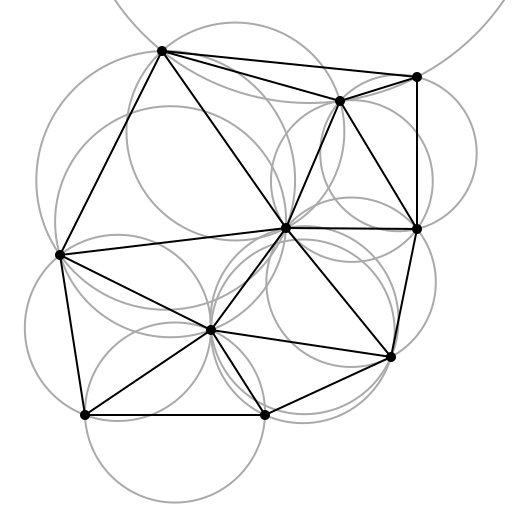
\includegraphics[width=1.25in]{images/illus_graphs/Delaunay_circumcircles_vectorial.png}}
    \boxed{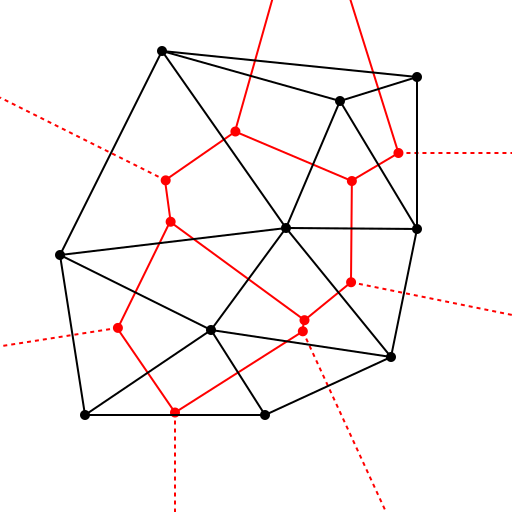
\includegraphics[width=1.25in]{images/illus_graphs/Delaunay_Voronoi.png}}
    \caption{Example of a Delaunay triangulation (in black) and Voronoi diagram (in red)}
    \label{fig:del_tri}
\end{figure}

\subsubsection{Gabriel graph}
A Gabriel graph \cite{10.2307/2412323} is a subgraph of a Delaunay triangulation. Thus, if the Delaunay triangulation is given, it can be found in a linear time. 

Formally, it is the graph in which any two distinct points $p, q \in P$ are adjacent precisely when the closed disc having $pq$ as a diameter contains no other points.

Basically, the interset of this method, compared to the Delaunay triangulation, is that it is adding a first level of filtration to suppress some neighbouring connexions.

\subsection{Finding real neighbours}
For the purpose of our experiments, i.e. finding \acrshort{bs} neighbours, the previously presented methods are not sufficient to find real neighbours.
As a consequence, some neighbouring connexions needs to be suppressed \cite{patent_neighs}.
\subsubsection{Distance criterion\cite{patent_neighs}}
A \acrshort{bs} does not have an infinite coverage area.
As a consequence, each edge in $U$ that is longer than a certain value, called \emph{max\_distance}, is suppressed.

\subsubsection{Angle criterion}
Let $p$, $q$, $r$ be three \acrshort{bs} of $P$, where $q$ and $r$ are $p$'s potential neighbours. As said before, coverage areas of \acrshort{bs} are limited by physics, this also implies that $r$ can be \og hidden\fg{} from $p$ by $q$ because $q$ is between $p$ and $r$ [trouver qqch pour prouver ce que je dis].

Therefore, the connexion between $p$ and $r$ needs to be suppressed. How? The angle $\widehat{qrp}$ is calculated and if it is narrower than a certain value, called \emph{min\_angle}, the longest edge is suppressed.

\subsubsection{Quadrant criterion}
As introduced in a previous article \cite{10201211} its goal is to prevent all potential neighbours to be in the same angle range. Therefore, it was mainly thought to be used with the 
$k$-NN potential neigbours method.

It consists in dividing the space around each base station into quadrants and keeping only a certain number of potential neighbours
in each of the quadrants, cf. Figure~\ref{fig:crit_qua}.
The number of quadrants has been fixed to six \cite{art_del_paq}.

\subsection{Density-based clustering methods}
\subsubsection{\acrshort{dbscan}}
\acrshort{dbscan} consists in detecting clusters based on the density of points, using two parameters:
\begin{itemize}
    \item \emph{$\varepsilon$}: A distance threshold under which two points are considered close enough to be considered neighbours;   
    \item \emph{$n_{\text{min}}$}: The shortest number of neigbours a points needs to have to be considered as a core point of a cluster.
\end{itemize}

The clusters will then \og grow\fg{} from the core points by attaching all points close from less than \emph{$\varepsilon$} than a point of the said 
cluster.

\subsubsection{\acrshort{hdbscan}}
\acrshort{hdbscan} \cite{10.1007/978-3-642-37456-2_14} is a variation of the \acrshort{dbscan} method. It consists
in selecting the best clusters after testing their persistence by making the $\varepsilon$ parameter vary. It's main particularity
is that it allows to detect clusters of different densities.

To each point who belongs to a cluster is associated a probability that symbolises the degree of certainty for this point to belong
to the said cluster.

\section{Contributions}
\noindent In section~\ref{sec:reminder}, we have seen that we can find the neighbours of base stations
by combining a potential neighbouring graph and filtration criteria. This methodology gives pretty good results \cite{art_del_paq}.

However, in certain cases like in a city, the filtration criteria aren't precise enough. We, therefore, need to find some ways to measure base stations' density.

\subsection{Measurement of \acrshort{bs} density}
Places with a high population also have a high density of base stations. In fact, each base station can only support a certain
load of users.

Therefore, we can assume that finding zones with a high density of base station is equivalent to finding the \acrshort{bs} 
situated in \og cities\fg{}.

\subsubsection{\acrshort{dbscan}}
DBScan gives only two categories : city - countryside
[permet de faire que 2 categories : pas assez précis (mais ptet à mettre dans résultats)]


\subsubsection{\acrshort{hdbscan}}
...

\subsubsection{$3$-NN mean distance}
For each base station $i$, the mean distance to its three nearest neighbours is calculated (we will call this value $\gamma_i$, in 
$\unit{km}$). According to the value of $\gamma_i$, the base station will be classified into a different category.

If you want this method to work properly, only \acrshort{bs} from the same provider have to be kept into the calculation process.
Althought this values are working well on France, we haven't tried yet on another country.

% \begin{itemize}
%     \item city center: $\gamma_i\in [0,1]$;
%     \item urban area: $\gamma_i\in ]1,2]$;
%     \item extra-urban: $\gamma_i\in ]2,4]$;
%     \item countryside: $\gamma_i\in ]4,\infty[$.
% \end{itemize}

\subsection{Improvement of filtering criteria}
\begin{table}
    \centering
    \caption{Summary of criteria values}
    \label{table:crit_summary}
    \begin{tabular}{lcc}
        \toprule
        \textbf{Description} & \textbf{\emph{max\_distance}} & \textbf{\emph{min\_angle}} \\
        \cmidrule(lr){1-3}
        city center & $\unit[2]{km}$ & $5^\circ$ \\
        urban area & $\unit[5]{km}$ & $10^\circ$ \\
        extra-urban area & $\unit[10]{km}$ & $15^\circ$ \\
        countryside & $\unit[15]{km}$ & $20^\circ$ \\
        \bottomrule
    \end{tabular}
\end{table}

\subsubsection{Distance and angle criterion}
As seen in section~\ref{sec:reminder}, after having found potential neighbours for each base station,
we need to filtrate this connexions. However, this applies the same distance and angle threshold for all base stations, without taking in account the difference of density.

The method we propose now is to take in account those differences of density for each site to apply a different threshold according to the category the site in classified in.

For both distance and angle, the more the base station is in a dense category, the lower this threshold will be.

\subsubsection{Quadrant criterion}
This criterion has been upgraded by adding the possibility to rotate the quadrants. The offset angle selected, which is between $0$ and 
$60$ degrees, is the one that maximises the sum of the distances of the potential neighbours to their closest quadrant delimitation.

In other words, it tends to select the angle with which the potential neighbors are as much in the middle of their respective quadrants
as possible.

The quadrant criterion is illustrated in Fig~\ref{fig:crit_qua}.
\begin{figure}
    \centering
    \boxed{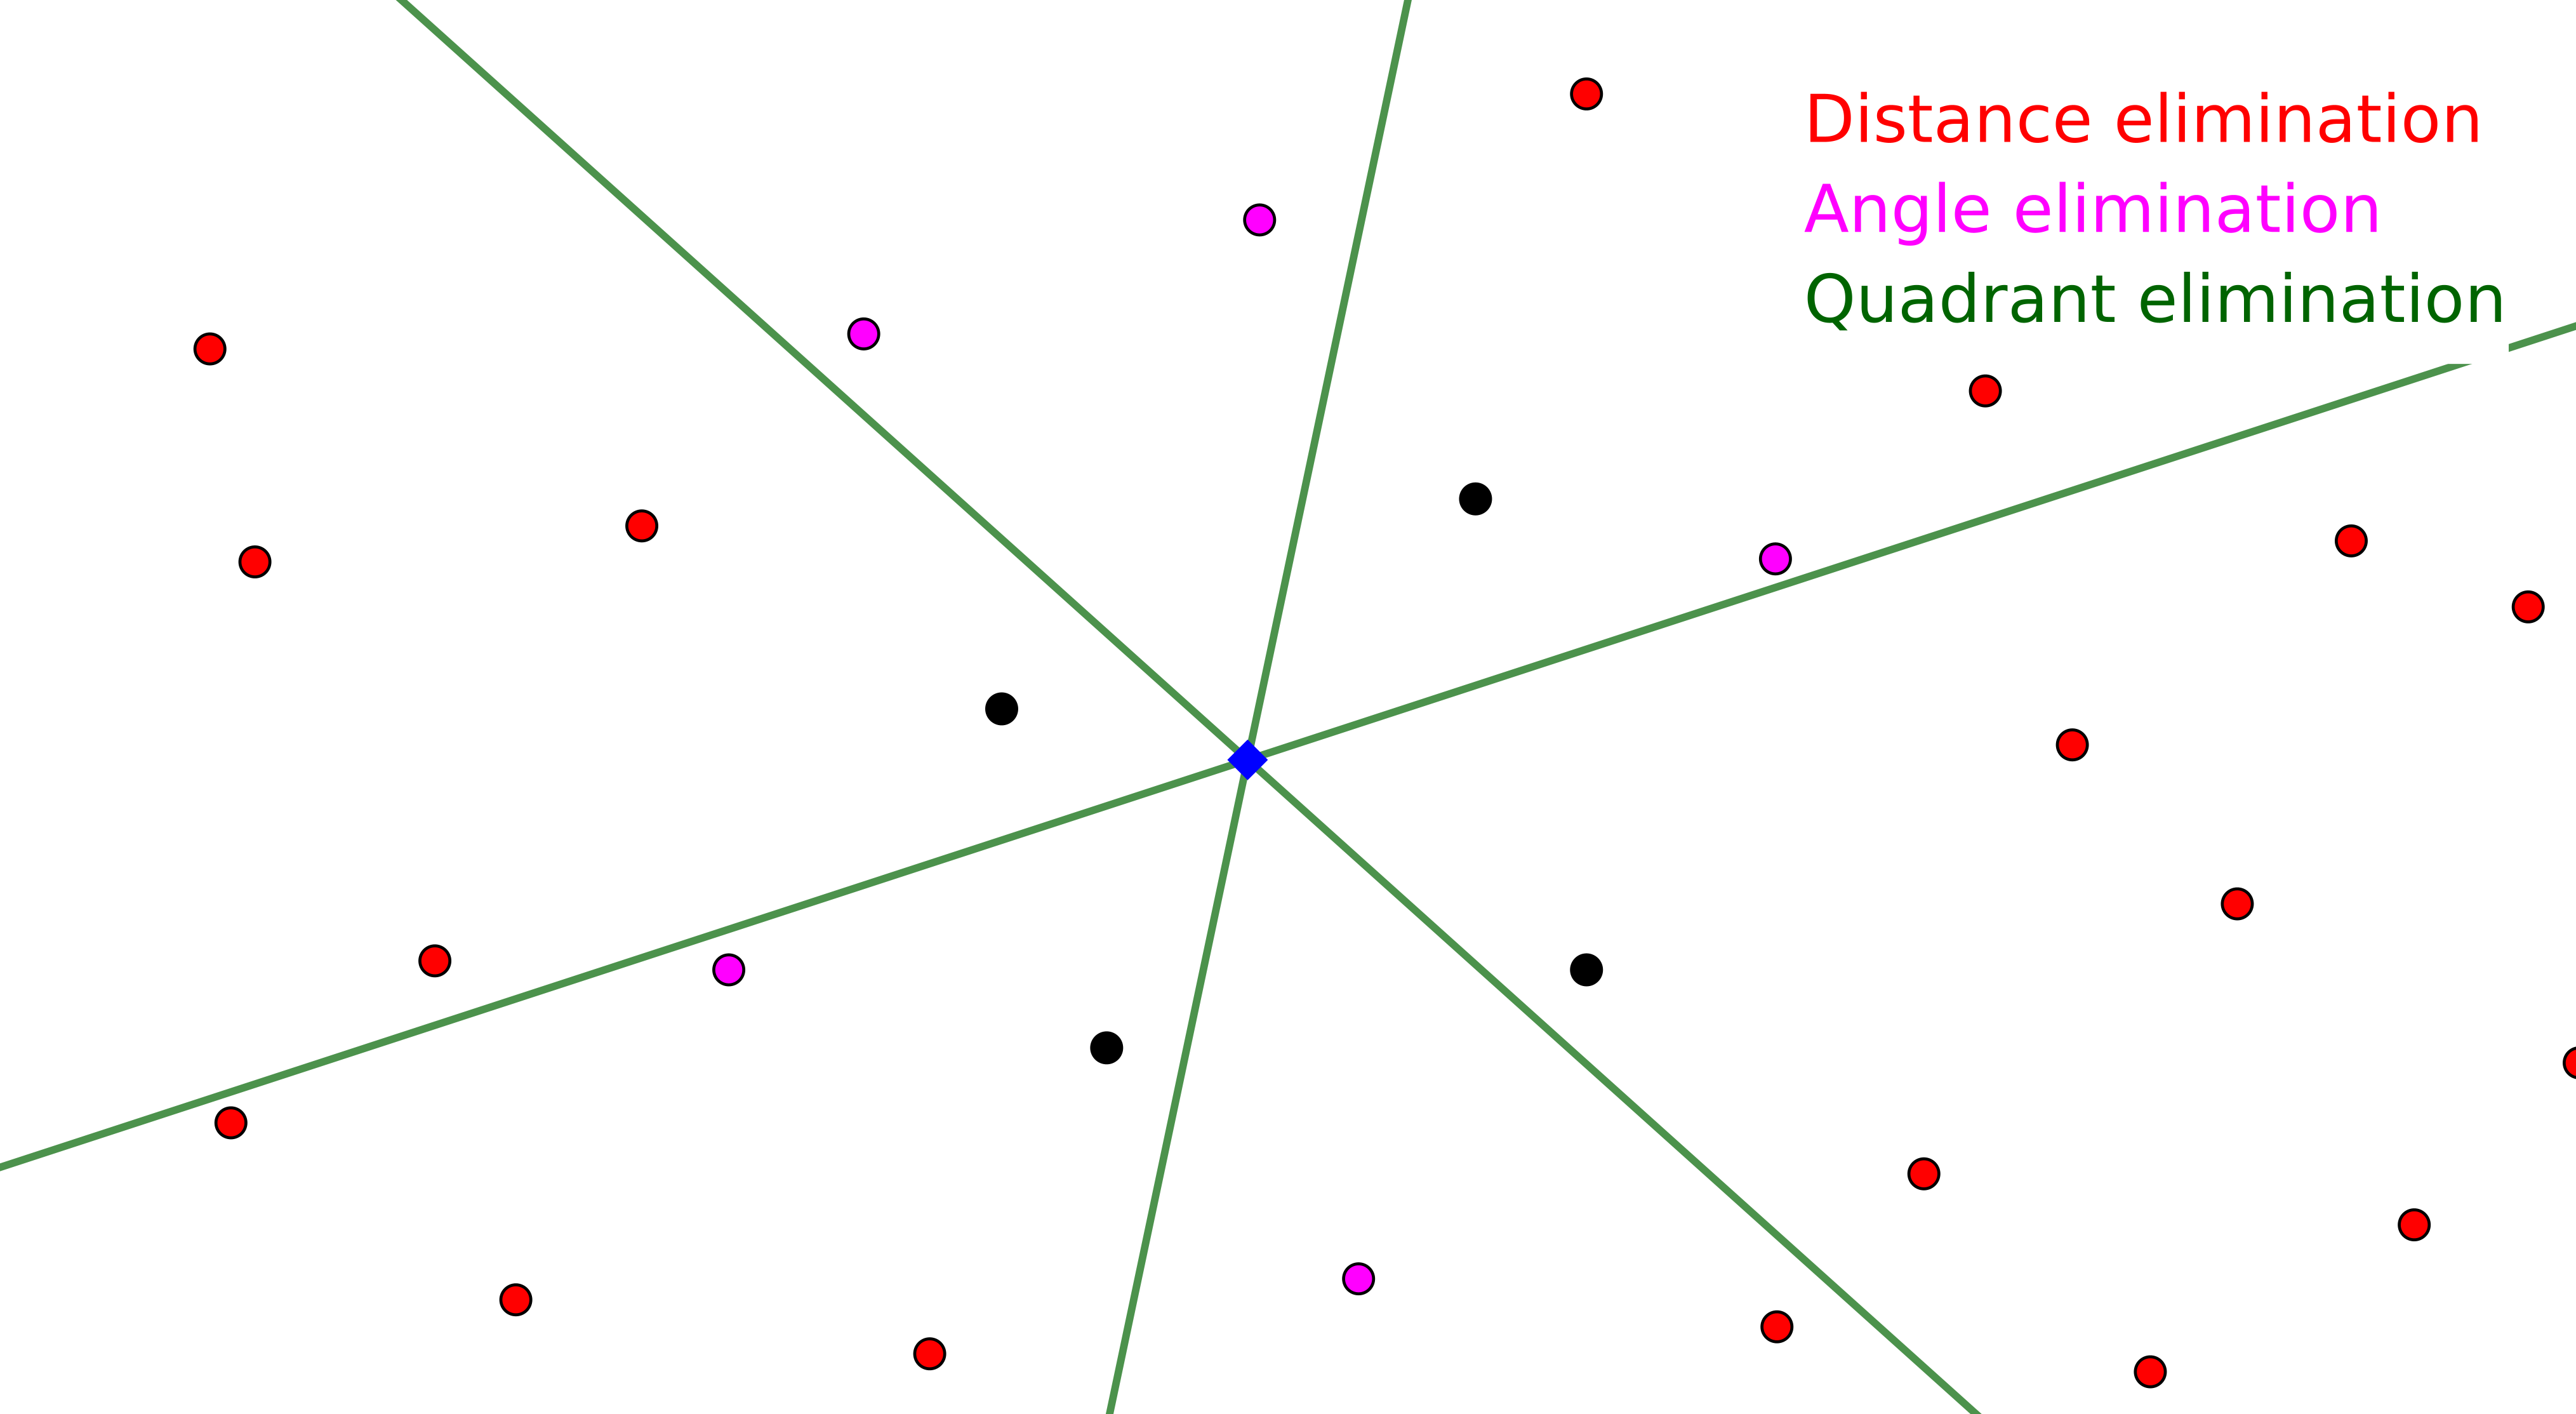
\includegraphics[width=2.5in]{images/illus_crit/quadrant_elim.png}}
    \caption{Illustation of the rotated quadrant criterion}
    \label{fig:crit_qua}
\end{figure}

\section{Results}

\subsection{Measurement of \acrshort{bs} density}

\subsection{Combining criteria}
As a matter of optimisation, criteria are applied one after another. For example, the base graph is Delaunay triangulation and we apply distance then angle.
The principle is that angle criterion will be applied on the Delaunay graph filtered with the distance criterion.

As a consequence, results differ according to the order in which the criteria are applied.

The best is Delaunay with distance and then angle.



\section{Conclusion}

[Ouverture: prendre en compte les zazimuths]

\printglossary[type=\acronymtype]
\printglossary

\bibliographystyle{IEEEtran}
\bibliography{./biblio.bib}

\end{document}


